%%%%%%%%%%%%%%
% The brew process
% Christopher Gandrud
% Updated 13 January 2012
%%%%%%%%%%%%%%

% Define colors for figure
%% Color palette (GnBU) chosen using ColorBrewer 2.0
%% See: http://colorbrewer2.org/
%% Not used in the print version
\definecolor{Blue}{HTML}{7BCCC4}
\definecolor{LiteBlue}{HTML}{A8DDB5}
\definecolor{DarkBlue}{HTML}{08589E}

\definecolor{GrayLine}{HTML}{BDBDBD}

% Set node styles
%% Workflow stage nodes
\tikzstyle{Docs} = [draw=Blue, 
                     rectangle, 
                     font=\scriptsize]

% Begin tikz picture
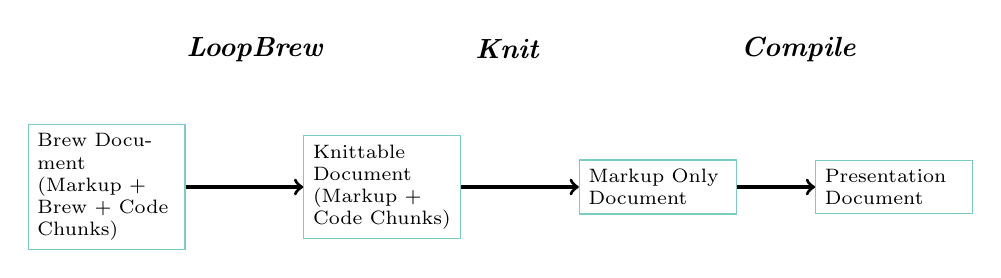
\begin{tikzpicture}
	
	\node(brew) at (1.9, 1.75) {{\emph{\textbf{Loop \\ Brew}}}};
	\node(knit) at (5.1, 1.75) {{\emph{\textbf{Knit}}}};
	\node(compile) at (8.8, 1.75) {{\emph{\textbf{Compile}}}};

	% Document nodes
	\node(brewable) at (0 , 0) [Docs, text width= 5em]{Brew Document \\ (Markup + Brew + Code Chunks)};
	\node (knittable) at (3.5, 0) [Docs, text width= 5em]{Knittable Document \\ (Markup + Code Chunks)};
	\node (Markup) at (7, 0) [Docs, text width= 5em]{Markup Only Document};
	\node (Presentation) at (10, 0) [Docs, text width = 5em]{Presentation Document};

	% Lines
	\draw [->, very thick] (brewable) -- (knittable);
	\draw [->, very thick] (knittable) -- (Markup);
	\draw [->, very thick] (Markup) -- (Presentation);


\end{tikzpicture}